\begin{figure}[h]
	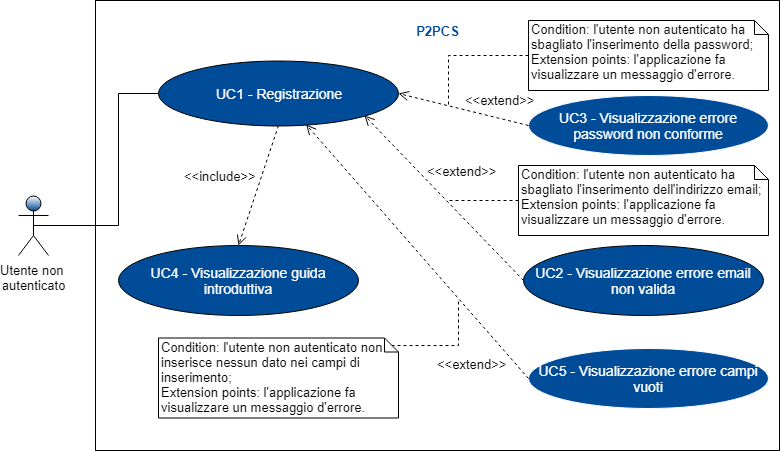
\includegraphics[width=15cm]{res/images/Schemagenerale1.png}
	\centering
	\caption{Diagramma del caso d'uso UC1 con relative estensioni (UC2, UC3, UC5) ed inclusioni (UC4)}
\end{figure}
\subsubsection{UC1 - Registrazione}
\begin{itemize}
	\item \textbf{Attori Primari}: utente non autenticato;
	\item \textbf{Descrizione}: per effettuare il procedimento di registrazione, l'utente deve compilare tutti i campi necessari ovvero nome, cognome, email, password e, se in possesso, anche del codice amico confermando i dati una volta inseriti per proseguire;
	\item \textbf{Scenario principale}: l'applicazione rende disponibili i campi da compilare per la registrazione. Dunque l'utente dovrà inserire tutti i dati necessari, quali:
		\begin{itemize}
			\item inserimento nome [UC1.1.1];
			\item inserimento cognome [UC1.1.2];
			\item inserimento indirizzo email [UC1.1.3];
			\item inserimento password [UC1.1.4];
			\item inserimento codice amico (solo se in possesso) [UC1.1.5].
		\end{itemize}
	Infine confermare i dati per procedere;
	\item \textbf{Precondizione}: l'applicazione rende disponibile i campi da compilare;
	\item \textbf{Postcondizione}: l'utente viene registrato nell'applicazione;
	\item \textbf{Inclusioni}:
		\begin{itemize}
			\item visualizzazione guida introduttiva [UC4].
		\end{itemize}
	\item \textbf{Estensioni}:
		\begin{itemize}
			\item visualizzazione errore email non valida [UC2];
			\item visualizzazione errore password non conforme [UC3];
			\item visualizzazione errore campi vuoti [UC5]. 
		\end{itemize} 
\end{itemize}
\begin{figure}[h]
	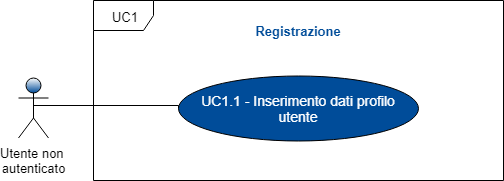
\includegraphics[width=10cm]{res/images/UC1Registrazione.png}
	\centering
	\caption{UC1 - Registrazione}
\end{figure}
\begin{figure}
	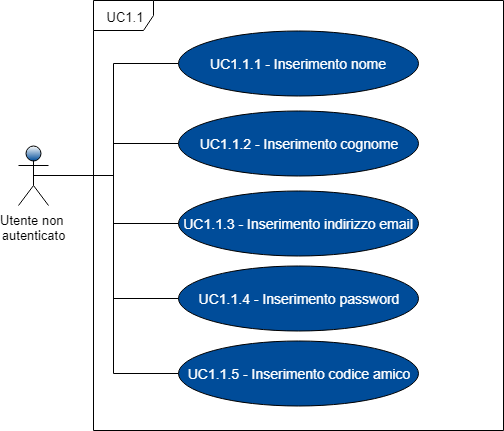
\includegraphics[width=9cm]{res/images/UC1-1Inserimento.png}
	\centering
	\caption{UC1.1 - Inserimento dati profilo utente}
\end{figure}
\subsubsection{UC1.1 - Inserimento dati profilo utente}
\begin{itemize}
	\item \textbf{Attori Primari}: utente non autenticato;
	\item \textbf{Descrizione}: l'utente compila i campi contenenti i dati relativi al profilo utente;
	\item \textbf{Scenario principale}: l'utente compila tutti i campi del form riguardanti l'account, ovvero:
		\begin{itemize}
			\item l'utente inserisce il proprio nome [UC1.1.1];
			\item l'utente inserisce il proprio cognome [UC1.1.2];
			\item l'utente inserisce l'email da associare all'account [UC1.1.3];
			\item l'utente inserisce la password da associare all'account [UC1.1.4];
			\item l'utente inserisce, solo se in possesso, il codice amico [UC1.1.5].
		\end{itemize}
	\item \textbf{Precondizione}: l'utente è entrato nell'activity\glosp di registrazione;
	\item \textbf{Postcondizione}: l'utente ha compilato tutti i campi richiesti dalla registrazione.
\end{itemize}
\newpage
\subsubsection{UC1.1.1 - Inserimento nome}
\begin{itemize}
	\item \textbf{Attori Primari}: utente non autenticato;
	\item \textbf{Descrizione}: al fine di portare a termine il processo di registrazione l'utente deve inserire il proprio nome, campo ritenuto obbligatorio;
	\item \textbf{Scenario principale}: l'utente compila il campo relativo al nome;	
	\item \textbf{Precondizione}: l'applicazione ha reso disponibile il campo per l'inserimento del nome;
	\item \textbf{Postcondizione}: l'utente ha compilato il campo con il proprio nome.	
\end{itemize}
\subsubsection{UC1.1.2 - Inserimento cognome}
\begin{itemize}
	\item \textbf{Attori Primari}: utente non autenticato;
	\item \textbf{Descrizione}: al fine di portare a termine il processo di registrazione l'utente deve inserire il proprio cognome, campo ritenuto obbligatorio;
	\item \textbf{Scenario principale}: l'utente compila il campo relativo al cognome;	
	\item \textbf{Precondizione}: l'applicazione ha reso disponibile il campo per l'inserimento del cognome;
	\item \textbf{Postcondizione}: l'utente ha compilato il campo con il proprio cognome.	
\end{itemize}
\subsubsection{UC1.1.3 - Inserimento indirizzo email}
\begin{itemize}
	\item \textbf{Attori Primari}: utente non autenticato;
	\item \textbf{Descrizione}: al fine di portare a termine il processo di registrazione l'utente deve inserire il proprio indirizzo email, campo ritenuto obbligatorio;
	\item \textbf{Scenario principale}: l'utente compila il campo relativo all'indirizzo email;	
	\item \textbf{Precondizione}: l'applicazione ha reso disponibile il campo per l'inserimento dell'indirizzo email;
	\item \textbf{Postcondizione}: l'utente ha compilato il campo con il proprio indirizzo email.
\end{itemize}
\subsubsection{UC1.1.4 - Inserimento password}
\begin{itemize}
	\item \textbf{Attori Primari}: utente non autenticato;
	\item \textbf{Descrizione}: al fine di portare a termine il processo di registrazione l'utente deve inserire una password, campo ritenuto obbligatorio;
	\item \textbf{Scenario principale}: l'utente compila il campo relativo alla password;	
	\item \textbf{Precondizione}: l'applicazione ha reso disponibile il campo per l'inserimento della password;
	\item \textbf{Postcondizione}: l'utente ha compilato il campo con una password.
\end{itemize}

\subsubsection{UC1.1.5 - Inserimento codice amico}
\begin{itemize}
	\item \textbf{Attori Primari}: utente non autenticato;
	\item \textbf{Descrizione}: al fine di portare a termine il processo di registrazione l'utente può inserire un "codice amico", qualora ne fosse in possesso, campo ritenuto non obbligatorio;
	\item \textbf{Scenario principale}: l'utente può compilare il campo relativo al codice amico se in possesso di un codice personale inviato da un altro utente che usufruisce dell'applicazione;	
	\item \textbf{Precondizione}: l'applicazione ha reso disponibile il campo per l'inserimento del codice amico;
	\item \textbf{Postcondizione}: l'utente ha compilato il campo con un codice amico.
\end{itemize}

%\subsubsection{UC1.2 - Invio dati}
%\begin{itemize}
%	\item \textbf{Attori Primari}: utente non autenticato;
%	\item \textbf{Descrizione}: l'utente non ancora autenticato, dopo aver inserito i dati per la registrazione, preme il pulsante per la conferma e l'invio dei dati; l'utente verrà rimandato a una nuova activity\glosp che confermerà il successo dell'operazione;
%	\item \textbf{Scenario principale}: l'utente non autenticato preme il pulsante di conferma ed invio dei dati;	
%	\item \textbf{Precondizione}: i campi dati necessari per la registrazione sono compilabili. È presente il pulsante per la conferma dei dati;
%	\item \textbf{Postcondizione}: l'utente, non ancora registrato, viene rimandato a una nuova activity che conferma il successo dell'operazione e avvisa l'utente di controllare la propria e-mail per confermare il processo di registrazione.
%\end{itemize}

\subsubsection{UC2 - Visualizzazione errore email non valida}
\begin{itemize}
	\item \textbf{Attori Primari}: utente non autenticato;
	\item \textbf{Descrizione}: l'utente visualizza un messaggio d'errore in quanto l'email digitata è scorretta;
	\item \textbf{Scenario principale}: l'utente non ancora autenticato tenta di registrarsi inserendo un indirizzo email non valido;
	\item \textbf{Precondizione}: l'utente non autenticato ha sbagliato l'inserimento dell'indirizzo email; 
	\item \textbf{Postcondizione}: l'applicazione fa visualizzare un messaggio d'errore.
\end{itemize}

\subsubsection{UC3 - Visualizzazione errore password non conforme}
\begin{itemize}
	\item \textbf{Attori Primari}: utente non autenticato;
	\item \textbf{Descrizione}: l'utente visualizza un messaggio d'errore in quanto la password digitata non è conforme ai seguenti vincoli:
		\begin{itemize}
			\item ci deve essere almeno una lettera maiuscola;
			\item ci deve essere almeno un carattere speciale;
			\item ci devono essere almeno 8 caratteri;
		\end{itemize}
	\item \textbf{Scenario principale}: l'utente non ancora autenticato tenta di registrarsi inserendo un password errata;
	\item \textbf{Precondizione}: l'utente non autenticato ha sbagliato l'inserimento della password; 
	\item \textbf{Postcondizione}: l'applicazione fa visualizzare un messaggio d'errore.
\end{itemize}

\subsubsection{UC4 - Visualizzazione guida introduttiva}
\begin{itemize}
	\item \textbf{Attori Primari}: utente non autenticato;
	\item \textbf{Descrizione}: l'utente visualizza una guida introduttiva che mostra le funzionalità dell'applicazione nella sue sezioni principali al termine della quale potrà accedere alla pagina di login;
	\item \textbf{Scenario principale}: l'utente accede alla guida introduttiva dell'applicazione e può decidere se visualizzarla o saltarla andando ad effettuare l'accesso;
	\item \textbf{Precondizione}: l'utente si è registrato e può accedere alla guida introduttiva dell'applicazione;
	\item \textbf{Postcondizione}: il sistema fornisce all'utente la possibilità di visualizzare interamente la guida o di saltarla e raggiungere la pagina di login.
\end{itemize}

\subsubsection{UC5 - Visualizzazione errore campi vuoti}
\begin{itemize}
	\item \textbf{Attori Primari}: utente non autenticato;
	\item \textbf{Descrizione}: l'utente visualizza un messaggio d'errore in quanto non sono stati riempiti i campi di inserimento email e password;
	\item \textbf{Scenario principale}: l'utente non ancora autenticato tenta di accedere non inserendo un indirizzo email e password;	
	\item \textbf{Precondizione}: l'utente non autenticato non inserisce nessun dato nei campi di inserimento;
	\item \textbf{Postcondizione}: l'applicazione fa visualizzare un messaggio d'errore.
\end{itemize}